% Dokumentinformationen
%Vorlage erstellt von Luca Mazzoleni aufbaudend auf der Vorlage von Stefan Reinli

% !TeX program = pdflatex
% !TeX encoding = utf8
% !TeX spellcheck = de_DE
% !BIB program = bibtex

\documentclass[
11pt,
final,
twoside,
a4paper]{article}
%%%%

% Document information
\newcommand*{\Title}            {Low Power wake up\\Receiver}
\newcommand*{\TitleInfo}        {Semesterarbeit HS 2019}
\newcommand*{\AuthorOne}		{Cédric Renda}
\newcommand*{\AuthorTwo}		{Manuel Tischhauser}
\newcommand*{\Author}			{\AuthorOne, \AuthorTwo}
\newcommand*{\Prof}				{Heinz Matthis}
\newcommand*{\Modul}			{Wireless Communication}
\newcommand*{\Betreuer}			{Heinz Matthis}
\newcommand*{\Place}            {Ort}
\newcommand*{\LogoHSR}          {
\includegraphics[height = 1cm]{header/hsrlogo}}
\newcommand*{\LogoCompany}      {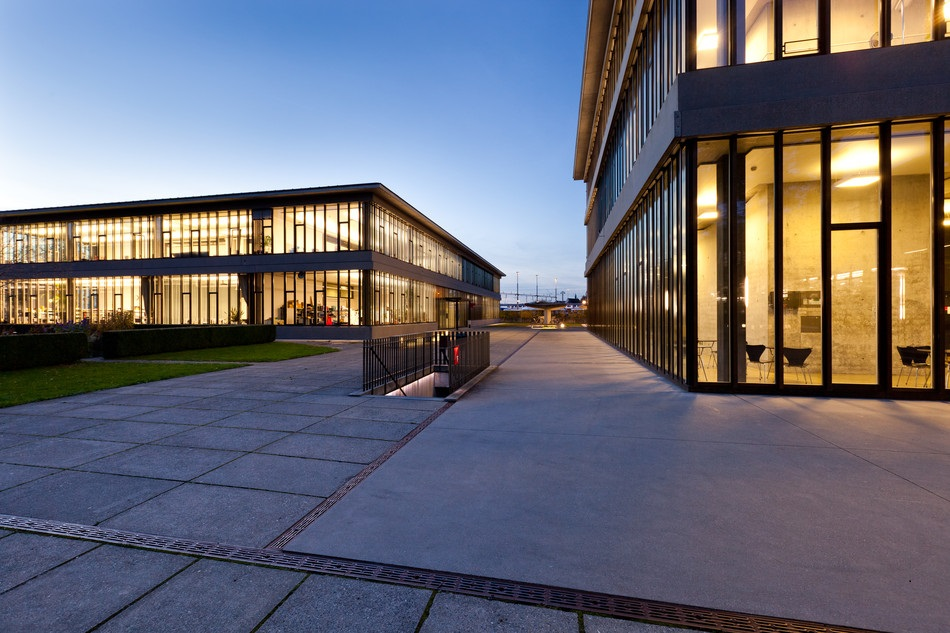
\includegraphics[height = 1cm]{header/logo}}
\newcommand*{\Print}            {false} % true for black links (print version), false for color links (pdf version)

% Header
%%%%%%%%%%%%%%%%%%%%%%%%%%%%%%%%%%%%%%%%%%
% Dokument
%%%%%%%%%%%%%%%%%%%%%%%%%%%%%%%%%%%%%%%%%%
% Geometrie
\newcommand{\paperFormat}{a4paper}
\newcommand{\lPageMargin}{20mm}
\newcommand{\rPageMargin}{20mm}
\newcommand{\tPageMargin}{20mm}
\newcommand{\bPageMargin}{20mm}

\documentclass[11pt,oneside]{scrartcl}

\newcommand{\newpar}{\par\par}

\usepackage[pdftitle={\titleinfo},%
			pdfauthor={\authorinfo},%
			pdfcreator={pdfLatex, LaTeX with hyperref},
			pdfsubject={\subjectinfo},
			plainpages=false,
			pdfpagelabels,
			colorlinks,
			linkcolor=black,
			filecolor=black,
			citecolor=black,
			urlcolor=black]{hyperref}
						

% Headings
\usepackage{scrlayer-scrpage}


%%%%%%%%%%%%%%%%%%%%%%%%%%%%%%%%%%%%%%%%%%
% Package's
%%%%%%%%%%%%%%%%%%%%%%%%%%%%%%%%%%%%%%%%%%
\usepackage{ucs}
\usepackage[utf8x]{inputenc}
\usepackage[T1]{fontenc}

\usepackage[free-standing-units=true, use-xspace=true]{siunitx}

\usepackage{layout}
\setlength{\parindent}{0em}

\renewcommand{\baselinestretch}{1.2}
\renewcommand{\arraystretch}{1}

%Damit \today ein Deutsch Formatiertes Datum zurueckgibt.
\usepackage[ngerman, num, orig]{isodate}
\usepackage[german, ngerman]{babel}
\monthyearsepgerman{\,}{\,}

\usepackage{amssymb,amsmath,fancybox,graphicx,wrapfig,color,lastpage,verbatim,epstopdf,a4wide,tabularx}
\usepackage{wasysym} %Checkboxen
\usepackage[usenames,dvipsnames]{pstricks}
\usepackage{setspace}
\usepackage{epsfig}
\usepackage{pst-pdf}
\usepackage{pst-all}
\usepackage{pstricks-add}
\usepackage{supertabular}
\usepackage[font=small,labelfont=bf]{caption}
\usepackage[font=footnotesize]{subfig}
\usepackage{footnote}
\usepackage{float}
\usepackage{multirow}
\usepackage{pdfpages}
\usepackage{pgf,tikz}
\usepackage{color}
\usepackage{titletoc}

\usepackage[makeroom]{cancel}
\usepackage{array}
\usepackage{trfsigns}
\usepackage{textcomp}

%Querformat
\usepackage{pdflscape}

\renewcommand{\captionfont}{\scriptsize\slshape}
	
\setlength{\unitlength}{1mm}

%Inhaltsverzeichnis
\setcounter{secnumdepth}{4}
\setcounter{tocdepth}{2}

%Geometrie
\usepackage[\paperFormat,left=\lPageMargin,right=\rPageMargin,top=\tPageMargin,bottom=\bPageMargin,includeheadfoot]{geometry}


%%%%%%%%%%%%%%%%%%%%%%%%%%%%%%%%%%%%%%%%%%%%%%%%%%%%%%%%%%%%%%%%
% Environment Numbering
%%%%%%%%%%%%%%%%%%%%%%%%%%%%%%%%%%%%%%%%%%%%%%%%%%%%%%%%%%%%%%%%

%Abbildungsnumerierung anhand Kapitel
\renewcommand{\thefigure}{\arabic{section}.\arabic{figure}}
\makeatletter \@addtoreset{figure}{section} \makeatother

%Gleichungen anhand Kapitel
\AtBeginDocument{\numberwithin{equation}{section}}
\AtBeginDocument{\numberwithin{figure}{section}}
\AtBeginDocument{\numberwithin{table}{section}}


%%%%%%%%%%%%%%%%%%%%%%%%%%%%%%%%%%%%%%%%%%%%%%%%%%%%%%%%%%%%%%%%
% Farben
%%%%%%%%%%%%%%%%%%%%%%%%%%%%%%%%%%%%%%%%%%%%%%%%%%%%%%%%%%%%%%%%
\definecolor{black}{rgb}{0,0,0}
\definecolor{red}{rgb}{1,0,0}
\definecolor{white}{rgb}{1,1,1}
\definecolor{grey}{rgb}{0.8,0.8,0.8}


%%%%%%%%%%%%%%%%%%%%%%%%%%%%%%%%%%%%%%%%%%%%%%%%%%%%%%%%%%%%%%%%
% Einheiten
%%%%%%%%%%%%%%%%%%%%%%%%%%%%%%%%%%%%%%%%%%%%%%%%%%%%%%%%%%%%%%%%


%Spannung
\DeclareMathOperator{\V}{\volt}
\DeclareMathOperator{\mV}{\milli \volt}
\DeclareMathOperator{\uV}{\micro \volt}

%Strom
\DeclareMathOperator{\A}{\ampere}
\DeclareMathOperator{\mA}{\milli \ampere}
\DeclareMathOperator{\uA}{\micro \ampere}
\DeclareMathOperator{\nA}{\nano \ampere}

%Zeit
\DeclareMathOperator{\s}{\second}
\DeclareMathOperator{\ms}{\milli \second}
\DeclareMathOperator{\us}{\micro \second}
\DeclareMathOperator{\ns}{\nano \second}

%Kapazitaet
\DeclareMathOperator{\mF}{\milli \farad}
\DeclareMathOperator{\uF}{\micro \farad}
\DeclareMathOperator{\nF}{\nano \farad}
\DeclareMathOperator{\pF}{\pico \farad}
\DeclareMathOperator{\fF}{\femto \farad}

%Induktivitaet
\DeclareMathOperator{\mH}{\milli \henry}
\DeclareMathOperator{\uH}{\micro \henry}
\DeclareMathOperator{\nH}{\nano \henry}

%Widerstand
\DeclareMathOperator{\MO}{\mega \ohm}
\DeclareMathOperator{\kO}{\kilo \ohm}
\DeclareMathOperator{\mO}{\milli \ohm}
\DeclareMathOperator{\Ohm}{\ohm}
%Strecke
\DeclareMathOperator{\km}{\kilo \meter}
\DeclareMathOperator{\cm}{\centi \meter}
\DeclareMathOperator{\mm}{\milli \meter}

%Frequenz
\DeclareMathOperator{\GHz}{\giga \hertz}
\DeclareMathOperator{\MHz}{\mega \hertz}
\DeclareMathOperator{\Hz}{\hertz}
\DeclareMathOperator{\kHz}{\kilo \hertz}
\DeclareMathOperator{\mHz}{\milli \hertz}

%Leistung
\DeclareMathOperator{\kW}{\kilo \watt}
\DeclareMathOperator{\mW}{\milli \watt}
\DeclareMathOperator{\uW}{\micro \watt}
\DeclareMathOperator{\W}{\watt}

%Kreisfrequenz
\DeclareMathOperator{\rpers}{\radianpersecond}

%DeziBel
\DeclareMathOperator{\dB}{\deci \bel}
\DeclareMathOperator{\dBm}{\deci \bel \milli}

%Bit
\DeclareMathOperator{\Bit}{\text{Bit}}
\DeclareMathOperator{\kBit}{\text{kBit}}
\DeclareMathOperator{\MBit}{\text{MBit}}
\DeclareMathOperator{\Byte}{\text{Byte}}
\DeclareMathOperator{\kByte}{\text{kByte}}
\DeclareMathOperator{\MByte}{\text{MByte}}
\DeclareMathOperator{\ppm}{\text{ppm}}
%%%%%%%%%%%%%%%%
% Code Layout %
%https://en.wikibooks.org/wiki/LaTeX/Source_Code_Listings
%%%%%%%%%%%%%%%

%\definecolor{mygreen}{rgb}{0,0.6,0}
%\definecolor{mygray}{rgb}{0.5,0.5,0.5}
%\definecolor{mymauve}{rgb}{0.58,0,0.82}

\lstset{ %
    firstnumber=1,
    backgroundcolor=\color{white},   % choose the background color; you must add        \usepackage{color} or \usepackage{xcolor}
    basicstyle=\footnotesize\ttfamily, % the size of the fonts that are used for the code
    breakatwhitespace=false,         % sets if automatic breaks should only happen at whitespace
    breaklines=true,                 % sets automatic line breaking
    captionpos=b,                    % sets the caption-position to bottom
    commentstyle=\color{mygreen},    % comment style
    deletekeywords={...},            % if you want to delete keywords from the given language
    otherkeywords={...},             % if you want to add more keywords to the set
    escapeinside={\%*}{*\%},          % if you want to add LaTeX within your code
    extendedchars=true,              % lets you use non-ASCII characters; for 8-bits encodings only, does not work with UTF-8
    frame=single,	                 % adds a frame around the code
    keepspaces=true,                 % keeps spaces in text, useful for keeping indentation of code (possibly needs columns=flexible)
    keywordstyle=\color{blue},       % keyword style
    language=C++,                    % the language of the code   
    numbers=left,                    % where to put the line-numbers; possible values are (none, left, right)
    numbersep=5pt,                   % how far the line-numbers are from the code
    numberstyle=\tiny\color{mygray}, % the style that is used for the line-numbers
    rulecolor=\color{black},         % if not set, the frame-color may be changed on line-breaks within not-black text (e.g. comments (green here))
    showspaces=false,                % show spaces everywhere adding particular underscores; it overrides 'showstringspaces'
    showstringspaces=false,          % underline spaces within strings only
    showtabs=false,                  % show tabs within strings adding particular underscores
    stepnumber=2,                    % the step between two line-numbers. If it's 1, each line will be numbered
    stringstyle=\color{mymauve},     % string literal style
    tabsize=2,	                     % sets default tabsize to 2 spaces
    %title=\lstname                   % show the filename of files included with         \lstinputlisting; also try caption instead of title
}

\lstdefinestyle{customc++}{
    belowcaptionskip=1\baselineskip,
    %frame=L,
    xleftmargin=\parindent,
    language=C++,
    keywordstyle=\bfseries\color{blue},
    commentstyle=\itshape\color{mygreen},
    identifierstyle=\color{black},
    stringstyle=\color{gray},
}

\lstdefinestyle{cppunit}{
    belowcaptionskip=1\baselineskip,
    %frame=L,
    xleftmargin=\parindent,
    language=C++,
    keywordstyle=\bfseries\color{blue},
    keywordstyle=[2]\bf\color{black}, %not sure why \bf works, but it does
    commentstyle=\itshape\color{mygreen},
    identifierstyle=\color{black},
    stringstyle=\color{gray},
    keywords=[2]{  %Cpp Unit Keywords
        CPPUNIT_ASSERT,
        CPPUNIT_TEST,
        CPPUNIT_TEST_EXCEPTION,
        CPPUNIT_TEST_END,
        CPPUNIT_TEST_SUITE,
        CPPUNIT_TEST_SUITE_REGISTRATION,
        CPPUNIT_TEST_SUITE_END},
}

\lstdefinestyle{cppqt}{
    belowcaptionskip=1\baselineskip,
    %frame=L,
    xleftmargin=\parindent,
    language=C++,
    keywordstyle=\bfseries\color{blue},
    keywordstyle=[2]\bfseries\color{red},
    commentstyle=\itshape\color{mygreen},
    identifierstyle=\color{black},
    stringstyle=\color{gray},
    keywords=[2]{           % qt-Keywords
		Qt,
        SIGNAL,
        SLOT,
        QApplication,
        QDialog,
        QGridLayout,
        QPushButton,
        QLabel,
        QVBoxLayout,
        QHBoxLayout,
        QWidget,
        QGroupBox,
        QFont,
        QLineEdit,
        QRadioButton,
        QPen,
        QRect,
        QPaintEvent,
        QBrush,
        QPixmap,
        QPainter,
        QString,
        QPoint,
        update()},
}

\lstdefinestyle{cdoxy}{
    belowcaptionskip=1\baselineskip,
    %frame=L,
    xleftmargin=\parindent,
    language=C++,  
    keywordstyle=\bfseries\color{blue},
    commentstyle=\itshape\color{mygreen},
    identifierstyle=\color{black},
    stringstyle=\color{gray},
    otherkeywords={           % DoxygenKeywords
        ...,
        ....,
        @mainpage,
        @file,
        @author,
        @version,
        @date,
        @bug,
        @brief,
        @extended,
        @param,
        @return,
        @warning,
        @note,
        @see},
}

\lstdefinestyle{custommatlab}{
	belowcaptionskip=1\baselineskip,
	%frame=L,
	xleftmargin=\parindent,
	language=Matlab,
	basicstyle=\footnotesize\ttfamily,
	keywordstyle=\bfseries\color{blue},
	commentstyle=\itshape\color{mygreen},
	identifierstyle=\color{black},
	stringstyle=\color{mylilas},
}

%choose customstyle in DOC with \lstinputlisting[style=custom]{path}
\lstset{style=customc++}

\setcounter{secnumdepth}{4}

%\includeonly{sections/Einleitung,sections/Einleitung1,sections/Verzeichnisse}


% tcolorbox setup
\tcbset{width=(\linewidth-1mm)/2,before=,after=\hfill,arc=0mm,
	colframe=red!50!black,colback=white,colback = red!10}

\newcommand{\hsp}{\hspace{20pt}}
\titleformat{\section}[hang]{\Huge\bfseries}{\thesection\hsp\textcolor{gray80}{|}\hsp}{0pt}{\Huge\bfseries}
\titleformat{\subsection}[hang]{\huge\bfseries}{\thesubsection\hsp\textcolor{gray60}{|}\hsp}{0pt}{\Large\bfseries}
\titleformat{\subsubsection}[hang]{\Large\bfseries}{\thesubsubsection\hsp\textcolor{gray40}{|}\hsp}{0pt}{\large\bfseries}
\titleformat{\paragraph}[hang]{\large\bfseries}{\theparagraph\hsp\textcolor{gray20}{|}\hsp}{0pt}{\large\bfseries}

% fontstyle
%\renewcommand\familydefault{\sfdefault}    % Arial

% Document=========================================
\begin{document}
    \pagenumbering{Roman}
    \thispagestyle{empty}
    \begin{titlepage}
	
	\begin{adjustwidth}{-25mm}{-45mm}
		%Seite einmitteln gemäss werten im geometry package:		
		\begin{adjustwidth}{65mm}{10mm}
			\textsf{
				%\textsf{	%sans serif schrift
				\vspace*{4cm}
				\begin{flushleft}
					\Huge \textbf{\Title}\\
					\vspace{.25cm}
					\Large \sffamily\TitleInfo \\
				\end{flushleft}
			}
		\end{adjustwidth}
		
		\begin{adjustwidth}{35mm}{40mm}	
			\vfill
			\large
			\textsf{\textbf{Autoren}}\\
			\textsf{\Author} \\
			\textsf{\textbf{Dozent}}\\
			\textsf{\Prof}\\
			\textsf{\textbf{Betreuer}}\\
			\textsf{\Betreuer}\\
			\textsf{\textbf{Modul}}\\
			\textsf{\Modul}\\
			\hfill\hbox{}\\
			\textsf{HSR Hochschule für Technik Rapperswil}\\
			\hfill\hbox{}\\
			\textsf{\today}
            \vspace{3cm}
		\end{adjustwidth}		
	\end{adjustwidth}
\end{titlepage}

    \clearpage \pagebreak
    \thispagestyle{empty}
    \listoftodos
    \cleardoublepage \pagebreak
    \pagenumbering{arabic}
    \setcounter{page}{1}
    \thispagestyle{empty}

\newgeometry{left=2cm,right=4cm,top=1cm,bottom=1cm,headsep=1.5cm, marginparwidth=30mm,marginparsep=3mm,includeheadfoot}
\savegeometry{margin}
	\thispagestyle{empty}
	\section*{\huge Abstract}

Lorem\marg{Ausgangslage} \todo{Abstract} ipsum dolor sit amet, consetetur sadipscing elitr, sed diam nonumy eirmod tempor invidunt ut labore et dolore magna aliquyam erat, sed diam voluptua. At vero eos et accusam et justo duo dolores et ea rebum. Stet clita kasd gubergren, no sea takimata sanctus est Lorem ipsum dolor sit amet. Lorem ipsum dolor sit amet, consetetur sadipscing elitr, sed diam nonumy eirmod tempor invidunt ut labore et dolore magna aliquyam erat, sed diam voluptua. At vero eos et accusam et justo duo dolores et ea rebum. Stet clita kasd gubergren, no sea takimata sanctus est Lorem ipsum dolor sit amet.
\\

Lorem\marg{Aufgabenstellung} ipsum dolor sit amet, consetetur sadipscing elitr, sed diam nonumy eirmod tempor invidunt ut labore et dolore magna aliquyam erat, sed diam voluptua. At vero eos et accusam et justo duo dolores et ea rebum. Stet clita kasd gubergren, no sea takimata sanctus est Lorem ipsum dolor sit amet. Lorem ipsum dolor sit amet, consetetur sadipscing elitr, sed diam nonumy eirmod tempor invidunt ut labore et dolore magna aliquyam erat, sed diam voluptua. At vero eos et accusam et justo duo dolores et ea rebum. Stet clita kasd gubergren, no sea takimata sanctus est Lorem ipsum dolor sit amet.
\\

Lorem\marg{Problemstellung} ipsum dolor sit amet, consetetur sadipscing elitr, sed diam nonumy eirmod tempor invidunt ut labore et dolore magna aliquyam erat, sed diam voluptua. At vero eos et accusam et justo duo dolores et ea rebum. Stet clita kasd gubergren, no sea takimata sanctus est Lorem ipsum dolor sit amet. Lorem ipsum dolor sit amet, consetetur sadipscing elitr, sed diam nonumy eirmod tempor invidunt ut labore et dolore magna aliquyam erat, sed diam voluptua. At vero eos et accusam et justo duo dolores et ea rebum. Stet clita kasd gubergren, no sea takimata sanctus est Lorem ipsum dolor sit amet.
\\

Lorem\marg{Vorgehen} ipsum dolor sit amet, consetetur sadipscing elitr, sed diam nonumy eirmod tempor invidunt ut labore et dolore magna aliquyam erat, sed diam voluptua. At vero eos et accusam et justo duo dolores et ea rebum. Stet clita kasd gubergren, no sea takimata sanctus est Lorem ipsum dolor sit amet. Lorem ipsum dolor sit amet, consetetur sadipscing elitr, sed diam nonumy eirmod tempor invidunt ut labore et dolore magna aliquyam erat, sed diam voluptua. At vero eos et accusam et justo duo dolores et ea rebum. Stet clita kasd gubergren, no sea takimata sanctus est Lorem ipsum dolor sit amet.
\\
 \todo[inline]{erkentnisse}
Lorem\marg{Wesentliche Erkenntnise} ipsum dolor sit amet, consetetur sadipscing elitr, sed diam nonumy eirmod tempor invidunt ut labore et dolore magna aliquyam erat, sed diam voluptua. At vero eos et accusam et justo duo dolores et ea rebum. Stet clita kasd gubergren, no sea takimata sanctus est Lorem ipsum dolor sit amet. Lorem ipsum dolor sit amet, consetetur sadipscing elitr, sed diam nonumy eirmod tempor invidunt ut 
\\


\newgeometry{left=2cm,right=2cm,top=1cm,bottom=1cm,headsep=1.5cm, marginparwidth=1mm,marginparsep=3mm,includeheadfoot} %Seitenränder Dokument ohne Titelblatt und Abstract
\savegeometry{no-margin}
	\begin{spacing}{1}
		\startcontents[sections]
		\printcontents[sections]{l}{1}{\setcounter{tocdepth}{4}\section*{Inhaltsverzeichnis}}	
	\end{spacing}
	\cleardoublepage 
	
\loadgeometry{margin}
	\include{sections/Aufgabenstellung}
%    \cleardoublepage
	\section{Einleitung}


Lorem\marg{Ausgangssituation} Lorem dolor sit amet, consetetur sadipscing elitr, sed diam nonumy eirmod tempor invidunt ut labore et dolore magna aliquyam erat, sed diam voluptua. At vero eos et accusam et justo duo dolores et \autocite[22]{Roppel2006} ea rebum. Stet clita kasd gubergren, no sea \textbf{\ref{tab:Hochwasserszenarien}} takimata sanctus est Lorem ipsum dolor sit amet. Lorem ipsum dolor sit amet, consetetur sadipscing elitr, sed diam nonumy eirmod tempor invidunt ut labore et dolore magna aliquyam erat, sed diam voluptua. At vero eos et accusam et justo duo dolores et ea rebum. Stet clita kasd gubergren, \textbf{\ref{fig:HSR}} no sea takimata sanctus est Lorem ipsum dolor sit\footcite{Roppel2006} \textbf{\ref{eq:Hochwasserzufluss}} amet.\footfullcite{Roppel2006}

\begin{figure}[ht]
	\centering
	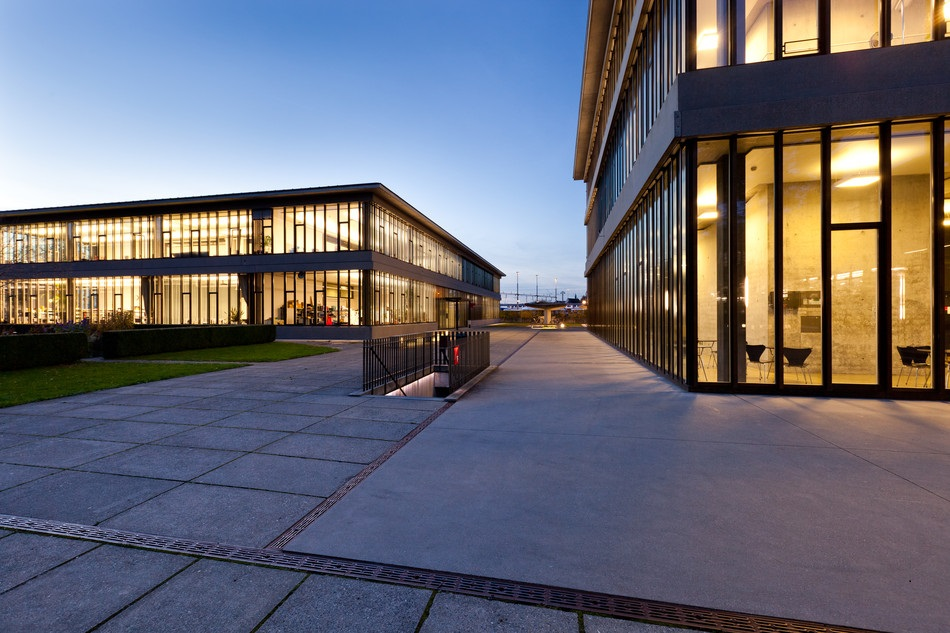
\includegraphics[width=0.6\textwidth]{images/hsr.jpg}
	\caption{\acs{HSR} \autocite{IR}}
	\label{fig:HSR}
\end{figure}

Lorem\marg{Was ist das Problem?}

 \begin{equation}\label{eq:Hochwasserzufluss}
\frac{Q(t)}{Q_{max}} = \left(\frac{t}{t_max}\cdot e^{1-\frac{t}{t_max}} \right)^n
\end{equation}
\myequations{Definition Hochwasserzufluss}

\begin{table}[ht]
    \centering
	\begin{tabular}{|l|l|l|l|l|l|}
		\hline 
		\textbf{Ganglinie}	&\textbf{[ ... ]}  	& \textbf{A} 	 & \textbf{B}  	& \textbf{C} 	& \textbf{D}  \\ 
		\hline 
		$ Q_{max} $			& $ m^3/s $ 		& 50 			& 70		  	& 180			& 540 \\ 
		\hline 
		$ t_{max} $			& $ h $ 			& 2  			& 2 			& 3 			& 4 \\ 
		\hline 
		n					& --  				& 6  			& 6 			& 6 			& 6  \\ 
		\hline 
	\end{tabular} 
	\caption{Hochwasserszenarien}\label{tab:Hochwasserszenarien}
\end{table}

Lorem \marg{Ziel} Lorem dolor sit amet, consetetur sadipscing elitr, sed diam nonumy ei\\

Lorem \marg{Wie soll das Problem gelöst werden?} Lorem dolor sit amet, consetetur sadipscing elitr, sed diam nonumy ei \\
\ac{HSR}\\
\acs{HSR}\\
\acl{HSR}


\clearpage
	\section{Evaluation}
This section lists the pros and cons of available Technologies.
On this basis was evaluated, which hardware is suitable.

\subsection{Energy harvesting}
\begin{tabularx}{\linewidth}{m{3cm}|X|X}
	\textbf{Technologie}&\textbf{Pro}&\textbf{Contra}\\
	\hline
	BLA&
	\begin{itemize}
		\item[-] bla
	\end{itemize}&
	\begin{itemize}
		\item[-] bla
	\end{itemize}\\
	\hline	
\end{tabularx}


\subsection{Wireless interface}
\begin{tabularx}{\linewidth}{m{3cm}|X|X}
	\textbf{Technologie}&\textbf{Pro}&\textbf{Contra}\\
	\hline
	Visual light communication&
	\begin{itemize}
		\item[-] Radiation is proper for any environment
		\item[-] High data rate (several Gb/s)
		\item[-] Light for transmission can also be used as energy resource
	\end{itemize}&
	\begin{itemize}
		\item[-] Only little products are available yet
		\item[-] Limited usability with existing lightning systems,  additional ethernet cables to lightbulbs may be required
		\item[-] Direct irradiation is needed
	\end{itemize}\\
	\hline
	Wake-up radio&
	\begin{itemize}
		\item[-] Range typically around 30m, but can be improved with antenna diversity and directional antennas
	\end{itemize}&
	\begin{itemize}
		\item[-] bla
	\end{itemize}\\	
\end{tabularx}


\subsection{Microcontroller}
\begin{tabularx}{\linewidth}{m{3cm}|X|X}
	\textbf{Technologie}&\textbf{Pro}&\textbf{Contra}\\
	\hline
	BLA&
	\begin{itemize}
		\item[-] bla
	\end{itemize}&
	\begin{itemize}
		\item[-] bla
	\end{itemize}\\
	\hline	
\end{tabularx}


	\section{Pflichtenheft}
Lorem\marg{Ausgangslage} \todo{Abstract} ipsum dolor sit amet, consetetur sadipscing elitr, sed diam nonumy eirmod tempor invidunt ut labore et dolore magna aliquyam erat, sed diam voluptua. At vero eos et accusam et justo duo dolores et ea rebum. Stet clita kasd gubergren, no sea takimata sanctus est Lorem ipsum dolor sit amet. Lorem ipsum dolor sit amet, consetetur sadipscing elitr, sed diam nonumy eirmod tempor invidunt ut labore et dolore magna aliquyam erat, sed diam voluptua. At vero eos et accusam et justo duo dolores et ea rebum. Stet clita kasd gubergren, no sea takimata sanctus est Lorem ipsum dolor sit amet.
\subsection{Bestandesaufnahme}
dd\marg{Ausgangslage}ff
\missingfigure{Test}
\subsubsection{Funktionsweise des Systems}
dd\marg{Ausgangslage}ff
\subsection{Anforderungen an das System}
dd\marg{Ausgangslage}ff
\subsubsection{Funktionsablauf}
dd\marg{Ausgangslage}ffv
v
\clearpage
	 \vspace{-3cm}
\section{Projektplan}
%{\centering
%	\vspace{-0.4cm}}
%	\includegraphics[angle=90,clip, trim= 0.5cm 5.5cm 1cm 2cm, scale=0.83]{sections/Projektterminplan_SA.pdf}\par}

	\section{Hauptstudie}
	\section{Fazit}
	
\loadgeometry{no-margin}
	\section{Erklärung zur Urheberschaft}
\vspace{0.8cm}
\textbf{Erklärung}\\

Wir erklären hiermit an Eides statt, dass ich die vorliegende Arbeit ohne Benutzung anderer als der angegebenen Hilfsmittel erstellt habe; die aus fremden Quellen direkt oder indirekt übernommenen Gedanken sind als solche kenntlich gemacht. Die Arbeit wurde bisher in gleicher oder ähnlicher Form keiner anderen Prüfungsbehörde vorgelegt und auch noch nicht veröffentlicht.\\
\vspace{0.8cm}\\

\begin{tabular}{l l}
    \textbf{Ort} & \textbf{Datum} \\
    \Place  & \today
\end{tabular}
\vspace{0.8cm}

\textbf{Unterschrift}\\
\vspace{0.2cm}
\AuthorOne \hspace{3cm} \AuthorTwo

\clearpage


	\section{Verzeichnisse}
%Abkürzungsverzeichniss, für schön ausrichten längste Abkürzung in eckige Klammer
\subsection{Abkürzungen}
\vspace{0.1cm}
\begin{acronym}[BA]
%\acro{Abkürzung}{Ausdruck ausgeschrieben}	
\acro{HSR}{Hochschule für Technik Rapperswil}
\end{acronym}	
\clearpage
\pagebreak


%Gleichungsverzeichnis
\subsection{\listequationsname}
\renewcommand*\listequationsname{}
\listofmyequations\thispagestyle{fancy}
\clearpage
\pagebreak

%Abbildungsverzeichnis
\subsection{\listfigurename}
\renewcommand*\listfigurename{}
\listoffigures\thispagestyle{fancy}
\clearpage
\pagebreak

%Tabellenverzeichnis
\subsection{\listtablename}
\renewcommand*\listtablename{}
\listoftables\thispagestyle{fancy}
\clearpage
\pagebreak

%Quellenverzeichnis
\subsection{Quellenverzeichnis}
\printbibliography[heading=subbibliography,keyword=lit, title={Literaturquellen}]
\printbibliography[heading=subbibliography,keyword=manual, title={Datenblätter}]
\printbibliography[heading=subbibliography,keyword=online, title={Onlinequellen}]
\printbibliography[heading=subbibliography,keyword=abb, title={Bildquellen}]

\clearpage
	\pagestyle{appendix}
	\section*{Anhang}
\addcontentsline{toc}{section}{Anhang}
\appendix
\startcontents[sections]
\printcontents[sections]{l}{1}{\setcounter{tocdepth}{2}}
\clearpage
\pagebreak


%\includepdf[pages={1},scale=0.95, pagecommand={\section{Anhangbsp mit PDF}},offset=0 -2cm]{sections/anhang/BA.pdf}

%\includepdf[pages={2-},scale=0.95, pagecommand={\thispagestyle{appendix}}]{sections/anhang/BA.pdf}

\section{Anhang 2}
	\cleardoublepage
\end{document}
